\documentclass[aspectratio=169]{beamer}
\usetheme{Madrid}
\setbeamertemplate{navigation symbols}{}
\usecolortheme{default}
\usepackage{graphicx}
\usepackage{caption}
\usepackage{booktabs}

% Ensure content doesn't overlap with bottom title bar
\setbeamersize{text margin left=0.3cm,text margin right=0.3cm}

\title{AI-based Damage Detection for Power Grid Equipment with SaaS-oriented Design}
\subtitle{Proposal Defense}
\author{Yujie Feng}
\institute{Supervisor: Jin Hou}
\date{}

% Customize footline with three adaptive columns: author/institute, title, page number
\setbeamertemplate{footline}
{
  \leavevmode%
  \hbox{%
  % Column 1: Author and Supervisor (left, natural width)
  \begin{beamercolorbox}[wd=0.3\paperwidth,ht=2.25ex,dp=1ex,left]{author in head/foot}%
    \usebeamerfont{author in head/foot}\hspace*{2ex}\insertshortauthor\hspace*{0.5em}\insertshortinstitute
  \end{beamercolorbox}%
  % Column 2: Title (center, flexible width)
  \begin{beamercolorbox}[wd=0.5\paperwidth,ht=2.25ex,dp=1ex,center]{title in head/foot}%
    \usebeamerfont{title in head/foot}\insertshorttitle
  \end{beamercolorbox}%
  % Column 3: Page number (right, natural width)
  \begin{beamercolorbox}[wd=0.2\paperwidth,ht=2.25ex,dp=1ex,right]{date in head/foot}%
    \usebeamerfont{date in head/foot}\insertframenumber{} / \inserttotalframenumber\hspace*{2ex}
  \end{beamercolorbox}%
  }%
  \vskip0pt%
}

\begin{document}

%------------------------------------------------
\begin{frame}
  \titlepage
\end{frame}

%------------------------------------------------
\begin{frame}
\frametitle{Project Vision: A Scalable SaaS Inspection Platform}
\vspace{-5pt}
\small
\begin{columns}
\column{0.32\linewidth}
\textbf{Multi-modal Inputs}
\begin{itemize}
  \item UAV RGB imagery
  \item Infrared imagery
  \item Sensor telemetry streams
  \item Historical inspection records
\end{itemize}

\column{0.36\linewidth}
\textbf{AI Platform Core}
\begin{itemize}
  \item SaaS backend
    \begin{itemize}
      \item unified auth / RBAC
      \item multi-tenant isolation
      \item task queue / data lake
    \end{itemize}
  \item AI model registry
    \begin{itemize}
      \item Module A: Bird Nest Detection (PoC)
      \item Module B: Oil Leak Detection (Planned)
      \item Module C: Infrared High-Temperature Detection (Planned)
    \end{itemize}
\end{itemize}

\column{0.32\linewidth}
\textbf{Enterprise Outputs}
\begin{itemize}
  \item Alert center \& dashboard
  \item Maintenance workorders
  \item Visual analytics portal
  \item API \& mobile integration
\end{itemize}
\end{columns}
\end{frame}

%------------------------------------------------
\begin{frame}
\frametitle{Accomplished (1): End-to-End PoC -- Module A}
\vspace{-5pt}
\begin{block}{Why start with bird-nest detection?}
\begin{itemize}
  \item High-frequency, high-risk issue with clear visual patterns; ideal to validate the pipeline.
\end{itemize}
\end{block}
\begin{block}{Vertical slice implemented}
\centering
\footnotesize
\resizebox{\linewidth}{!}{%
  \begin{tabular}{c c c c c c c}
    \textbf{1. Data} & $\Rightarrow$ & \textbf{2. Training} & $\Rightarrow$ & \textbf{3. Engineering Optimizations} & $\Rightarrow$ & \textbf{4. Deployment} \\
    (43 train / 11 val) & & Mask R-CNN fine-tuning & & (DataLoader, AMP, Schedulers) & & (Flask microservice)
  \end{tabular}%
}
\end{block}
\end{frame}

%------------------------------------------------
\begin{frame}
\frametitle{PoC Progress (1): Training Results \& Metrics}
\vspace{-5pt}
\begin{columns}
\column{0.48\linewidth}
\textbf{COCO Validation Metrics}
\small
\begin{center}
\begin{tabular}{lcc}
\toprule
Metric & \textbf{bbox} & \textbf{segm} \\
\midrule
AP@[0.50:0.95] & 0.805 & 0.795 \\
AP50 & 1.000 & 1.000 \\
AP75 & 1.000 & 0.919 \\
AR@[0.50:0.95] & 0.837 & 0.828 \\
\bottomrule
\end{tabular}
\end{center}

\column{0.48\linewidth}
\textbf{Training Configuration}
\begin{itemize}
  \item Model: Mask R-CNN (ResNet50 + FPN v2)
  \item Dataset: 54 images (43 train, 11 val)
  \item Input size: 512$\times$512, batch size 4
  \item Optimizer: AdamW (lr=$5\cdot10^{-4}$), OneCycleLR
  \item Epochs: 40 (early-stop ready)
\end{itemize}
\end{columns}
\end{frame}

%------------------------------------------------
\begin{frame}
\frametitle{PoC Progress (2): Training Dynamics}
\vspace{-5pt}
\begin{columns}
\column{0.48\linewidth}
\centering
\includegraphics[width=0.95\textwidth]{../visualizations/loss_curves.png}
\vspace{-5pt}
\captionof{figure}{Train/Validation Loss}

\column{0.48\linewidth}
\textbf{Key Observations}
\begin{itemize}
  \item Loss drops from 1.41 to 0.14 (train), 0.65 to 0.19 (val)
  \item Plateaus around epoch 20
  \item GPU utilization: 70--85\% (after optimization)
  \item $\sim$ About 27 seconds per epoch
\end{itemize}
\end{columns}
\end{frame}

%------------------------------------------------
\begin{frame}
\frametitle{PoC Progress (3): Precision-Recall Analysis}
\vspace{-5pt}
\begin{columns}
\column{0.48\linewidth}
\centering
\includegraphics[width=0.95\textwidth]{../visualizations/pr_curve_bbox_ap50.png}
\vspace{-5pt}
\captionof{figure}{PR Curves (Bbox, IoU=0.50/0.75/0.90)}

\column{0.48\linewidth}
\centering
\includegraphics[width=0.95\textwidth]{../visualizations/pr_curve_segm_ap50.png}
\vspace{-5pt}
\captionof{figure}{PR Curves (Segm, IoU=0.50/0.75/0.90)}
\end{columns}
\vspace{2pt}
\small
\textit{IoU=0.50 stays close to precision 1.0; IoU=0.75 settles around 0.93, while IoU=0.90 dips toward 0.70, showing localization sensitivity.}
\end{frame}

%------------------------------------------------
\begin{frame}
\frametitle{PoC Progress (4): IoU Distributions \& Threshold Analysis}
\vspace{-5pt}
\begin{columns}
\column{0.48\linewidth}
\centering
\includegraphics[width=0.85\textwidth]{../visualizations/iou_hist_bbox.png}
\vspace{-5pt}
\captionof{figure}{Bbox IoU Histogram}

\column{0.48\linewidth}
\centering
\includegraphics[width=0.85\textwidth]{../visualizations/threshold_sweep_bbox.png}
\vspace{-5pt}
\captionof{figure}{Score Threshold vs P/R/F1 (IoU$\geq$0.5)}
\end{columns}
\vspace{2pt}
\small
\textit{Right-skewed IoU mass indicates strong localization. With AP$_{50}$=1.0, precision remains high across thresholds; threshold 0.4--0.5 optimizes F1, while higher thresholds (0.6--0.8) maintain high precision with reduced recall.}
\end{frame}

%------------------------------------------------
\begin{frame}
\frametitle{PoC Progress (5): Production-Ready Microservice}
\vspace{-5pt}
\begin{columns}[T]
\column{0.48\linewidth}
\textbf{Flask REST API Features}
\begin{itemize}
  \item Batch image upload (multiple files)
  \item Real-time inference with visualization
  \item Interactive web interface
  \item Download results (single \& ZIP)
  \item Statistical dashboards \& charts
  \item Memory-optimized for large images
\end{itemize}

\column{0.48\linewidth}
\textbf{Platform Significance}
\begin{itemize}
  \item Demonstrates ``model as a service''
  \item First entry in AI model registry
  \item Production-ready with error handling
  \item Scalable architecture for multi-tenant SaaS
  \item User-friendly interface for field operators
\end{itemize}
\end{columns}
\vspace{8pt}
\begin{columns}[T]
\column{0.48\linewidth}
\centering
\includegraphics[width=0.95\textwidth,height=0.32\textheight,keepaspectratio]{flask-deploy-image.png}
\vspace{-3pt}
\captionof{figure}{Multiple Images Detection}

\column{0.48\linewidth}
\centering
\includegraphics[width=0.95\textwidth,height=0.32\textheight,keepaspectratio]{flask-deploy-image1.png}
\vspace{-3pt}
\captionof{figure}{Real-time Inference \& Visualization}
\end{columns}
\end{frame}

%------------------------------------------------
\begin{frame}
\frametitle{Key Insight: Generalization is the Core Challenge}
\vspace{-5pt}
\begin{block}{The Trap of a "Perfect" Score}
\begin{itemize}
  \item AP$_{50}=1.0$, IoU $\approx 1.0$ because validation data mirrors training scenes
  \item In real operations (fog, backlight, new structures) accuracy might drop sharply
\end{itemize}
\end{block}
\begin{block}{Platform Lesson}
\begin{itemize}
  \item Any module (nest, oil leak, high-temperature) must solve generalization to new conditions
  \item Data augmentation, negative sampling, and multi-scene evaluation are platform-level requirements
\end{itemize}
\end{block}
\end{frame}

%------------------------------------------------
\begin{frame}
\frametitle{Next Steps: Build Horizontally, Expand Vertically}
\vspace{-5pt}
\begin{columns}
\column{0.48\linewidth}
\textbf{Track 1 -- SaaS Platform (Weeks 4--10)}
\begin{itemize}
  \item Goal: Establish core infrastructure and standards
  \item Tasks:
    \begin{enumerate}
      \item Implement multi-tenant backend with RBAC and task orchestration
      \item Define APIs for the AI model registry
      \item Productize PoC training utilities (augmentation, logging)
    \end{enumerate}
\end{itemize}

\column{0.48\linewidth}
\textbf{Track 2 -- New Modules (Weeks 11--18)}
\begin{itemize}
  \item Goal: Validate extensibility
  \item Tasks:
    \begin{enumerate}
      \item Kick off Module B (oil leak detection) or Module C (infrared high-temperature detection)
      \item Reuse platform capabilities for data processing and training
      \item Onboard new modules into the registry and microservice catalog
    \end{enumerate}
\end{itemize}
\end{columns}
\end{frame}

%------------------------------------------------
\begin{frame}
\frametitle{Work Plan and Schedule}
\vspace{-5pt}
\centering
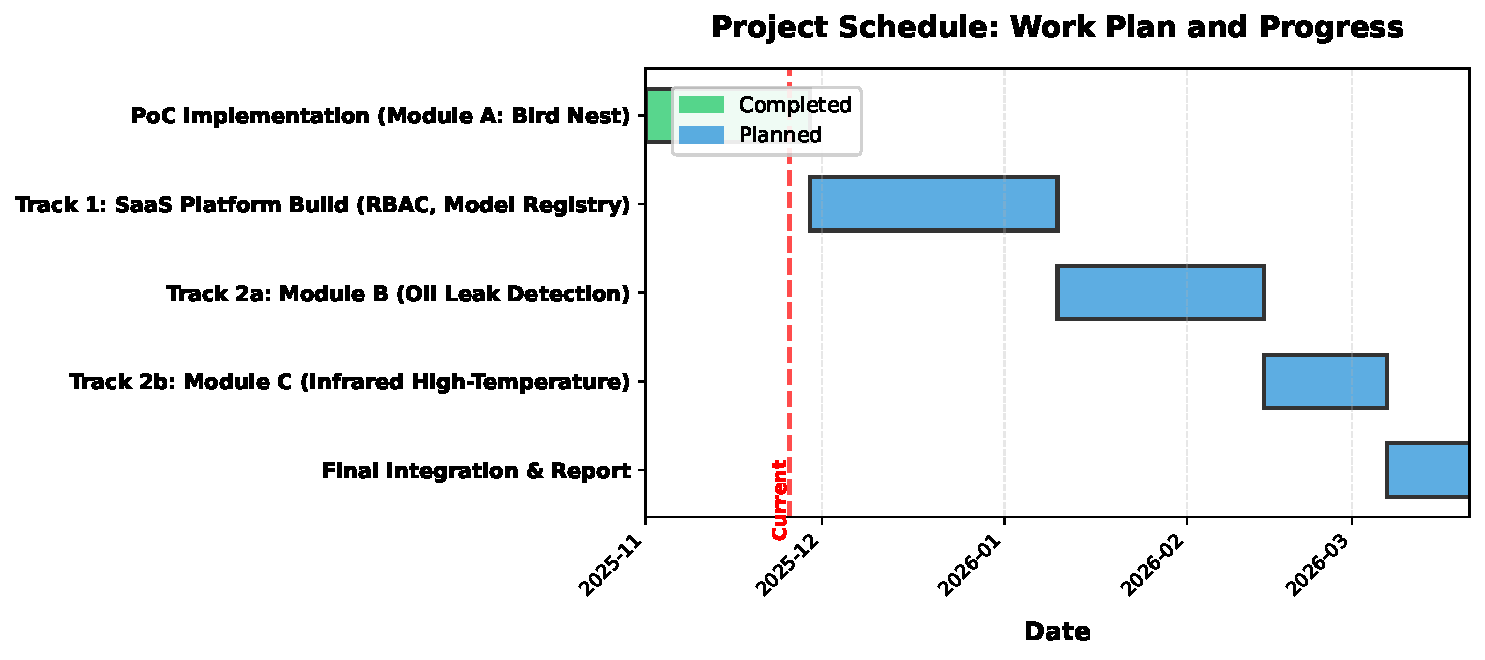
\includegraphics[width=0.85\textwidth,height=0.5\textheight,keepaspectratio]{project_schedule_gantt.png}
\vspace{3pt}
\footnotesize
\textbf{Two-Track Approach:}
\begin{itemize}
  \item {\color{green!70!black}Weeks 1--4 (Completed):} PoC Implementation (Module A)
  \item {\color{blue!70!black}Weeks 5--10:} Track 1 -- SaaS Platform Build
  \item {\color{blue!70!black}Weeks 11--15:} Track 2a -- Module B (Oil Leak)
  \item {\color{blue!70!black}Weeks 16--18:} Track 2b -- Module C (Infrared)
  \item {\color{blue!70!black}Weeks 19--20:} Final Integration \& Report
\end{itemize}
\end{frame}

%------------------------------------------------
\begin{frame}
\frametitle{Discussion Points}
\vspace{-5pt}
\begin{enumerate}
  \item SaaS backend depth: should I prioritize feature completeness first (prototype RBAC) or invest in production-grade auth from day one?
  \item Module B technical choices: oil leak detection may require different approaches—should I consider semantic segmentation (e.g., U-Net) or stick with instance segmentation?
  \item Module C integration: infrared high-temperature detection—should it be a standalone module or fused with RGB-based detection for multi-modal analysis?
\end{enumerate}
\end{frame}

\end{document}

